\documentclass[dvipdfmx, 12pt]{beamer}
\usepackage{pxjahyper}
\usepackage{minijs}
\usepackage{otf}
\renewcommand{\kanjifamilydefault}{\gtdefault}
\usetheme{Antibes}
\setbeamertemplate{navigation symbols}{}
\usepackage{url}
\usepackage{graphicx}
\usepackage{amsmath}
\usepackage{bm}
\usepackage{ascmac}
\setbeamertemplate{footline}[frame number] 


\title{Understanding Financial Crises\\Ch10 : Contagion 後半}
\author{Kei Ikegami}

\begin{document}
\newcommand{\argmin}{\mathop{\rm arg~min}\limits}

\frame{\maketitle}

\section*{目次}
\begin{frame} \frametitle{発表の流れ}
\tableofcontents
\end{frame}

\begin{frame}\frametitle{何をするか}
	\begin{itemize}
	\item 銀行間のつながりがincomplete networkでもfirst bestを達成することはできた。しかし世界全体での流動性需要量が想定される量よりも多くなる想定外の事象の下では、incomplete networkだとbankruptが地域を超えて連鎖するContagionが発生する。ということの確認。
	\item Contagionが全地域に拡大すると世界に存在する資産の価値が低下するのでやだ!ということの確認。
	\item 銀行のデータを使ってContagionが発生する規模をシミュレーションする研究の紹介。
	\end{itemize}
\end{frame}

\begin{frame}\frametitle{Pecking Order}
	\begin{itemize}
	\item date1において流動性需要が発生したときに、当該地域の銀行はどのようにして対処するかを考える。
	\item 銀行の持ってる資産は、short asset ($y$), 他銀行へのdeposits ($z$), long asset ($x$)の三種類。
	\item この三つをそれぞれ流動化して流動性を供給するわけだが、この三つは無差別ではない。
	\end{itemize}
\end{frame}

\begin{frame}\frametitle{Pecking Order : Cost of short asset}
	\begin{itemize}
	\item short assetを流動化する際のコストを考える。
	\item date 1で1の消費をもたらすshort assetの量は1である。
	\item このdate1で1の消費をもたらすだけのshort assetを使ってdate2で消費しようとすれば、買い替えによってdat2でも1だけの消費をすることができる。
	\item つまり、date1で1の消費を得るのにdate2での1を犠牲にしている。
	\item これよりshort assetを流動化するコストは1である。
	\end{itemize}
\end{frame}

\begin{frame}\frametitle{Pecking Order : Cost of depoists}
	\begin{itemize}
	\item 他国へのdepositsを流動化する際のコストを考える。
	\item interbank市場においても各国の消費者と銀行が結ぶのと同様の契約によって預金がなされているとする。
	\item すなわち、ある銀行がdate0において1単位の財を他国の銀行に預けるということは、預けた先の銀行からdate1では$c_1$、date2では$c_2$だけの引き出しを保証されているということである。
	\item ということは、date1で$c_1$だけの流動性を供給した場合、date2での$c_2$だけの消費を犠牲にしたということになる。
	\item 従ってdepositsを流動化するコストは単位あたり$\frac{c_2}{c_1}$である。
	\end{itemize}
\end{frame}

\begin{frame}\frametitle{Pecking Order : Cost of long asset}
	\begin{itemize}
	\item long assetを流動化する際のコストを考える。
	\item short assetの時と同様に考えれば良い。
	\item date1で$r$だけの消費を供給できるだけのlong assetは、date2まで持っておけば$R$だけの消費をもたらすことができるものである。
	\item 従ってlong assetを流動化するコストは単位あたり$\frac{R}{r}$である。
	\end{itemize}
\end{frame}

\begin{frame}\frametitle{Pecking Order}
	\begin{itemize}
	\item 当然先の三つをコストが安い順に流動化していく。
	\item 銀行のFOCより$1 < \frac{c_2}{c_1}$である。
	\item $r$を十分低く設定すれば$\frac{c_2}{c_1} < \frac{R}{r}$は満たされる。
	\item よって、以下では「short asset」「他銀行へのdeposits」「long asset」の順で流動化していくと仮定する。
	\item これをPecking orderと呼ぶ。
	\end{itemize}
\end{frame}

\begin{frame}\frametitle{設定1}
	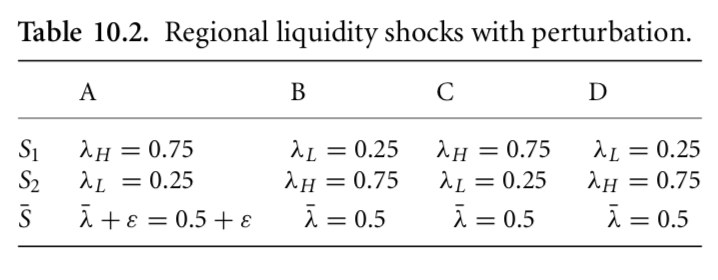
\includegraphics[width = 7cm]{10-2.png}
	
	\begin{itemize}
	\item $\bar{S}$が確率0で発生すると想定されている事象(本当はおこりうる)。
	\item $\epsilon$分だけ世界全体での流動性需要が通常の状態よりも多くなって老いることに注意。
	\end{itemize}
\end{frame}

\begin{frame}\frametitle{設定2}
	\begin{itemize}
	\item interbank networkは上図のようなincomplete netwrokとなっている。
	\item 異常事態$\bar{S}$には各主体確率0を割り当てているので、$z = 0.25$だけのdepositsを矢印の向きに預けている状態である。
	\end{itemize}
\end{frame}

\begin{frame}\frametitle{}
	\begin{itemize}
	\item 
	\end{itemize}
\end{frame}

\begin{frame}\frametitle{}
	\begin{itemize}
	\item 
	\end{itemize}
\end{frame}

\begin{frame}\frametitle{}
	\begin{itemize}
	\item 
	\end{itemize}
\end{frame}

\begin{frame}\frametitle{}
	\begin{itemize}
	\item 
	\end{itemize}
\end{frame}

\begin{frame}\frametitle{}
	\begin{itemize}
	\item 
	\end{itemize}
\end{frame}
\end{document}
